\chapter{Graph Experiments}

\textbf{\#TODO: run these again}
\textbf{\#TODO: copy metrics from plots}

As part of our research into more efficiently matching founder with investors, we sought to quantitatively demonstrate some of the commonly-accepted characteristics of fundraising. Furthermore, we wish to explore how we can leverage automated ranking systems to more appropriately match companies with a source of funding. To do this, we ran various experiments on a social graph of founders, investors, and their mutual connections. This graph is built from the information provided by founders on the VCWiz platform.

As discussed in the previous chapter, one of the features of VCWiz is a CRM for founders, which integrates with their inbox and scans (the headers of) all their emails back and forth with investors registered on the platform. As part of this optional integration, founders gave permission to have their aggregate email data used for research. As we scan these emails (filtering out any irrelevant ones, as described in Listing \ref{code:parse}), we build up a graph, where each node represents an individual (using their email as a unique key), and each edge represents an email connection between two nodes. Edges are directed: there exists an edge from node $i$ to node $j$ if and only if an email has been sent from email $e_i$ to email $e_j$. Edges have weights equal to the total such number of emails sent. In order to comply with the privacy provisions made to founders, we avoided more sophisticated weighting schemes involving features extracted from the email body. These weights are ignored when doing manipulations and calculating graph metrics, unless explicitly specified.

Our motivation for modeling the underlying graph for these experiments is as follows. The majority of pre-pitch and post-pitch communication when fundraising happens over email, and almost every introduction made to an investor on behalf of a founder is done by email as well. Furthermore, emails are often sent as follow-ups to in-person meetings (at networking events, etc.). Finally, email is the preferred medium for ongoing communication between and founder and their investors. Thus, by capturing the entirety of the email graph for the subset of founders and investors on our platform, we get an accurate picture of what relationships are at play.

\section{Experiments}

The remainder of this chapter will delve into the details of several experiments. The goal of these experiments is to better identify what correlates with a successful fundraise, and how we can use this information to better match founders and investors, for the purpose of maximizing funding likelihood.

It has long been supposed that the characteristics of a founder in his or her professional network can impact, and indeed predict, how successful a fundraising attempt will be. For the purposes of these experiments, we will define success as raising at least as much money as planned, from a founder's top pick of investors, in as short a time as possible. There is lots of anecdotal evidence to support these claims\footnote{https://about.crunchbase.com/blog/fundraising-dos-and-donts/}, and recently there has been statistical evidence as well. A 2017 study uses AngelList data ``to estimate the effects of network distance in the matches resulting from Series A financing rounds'', and concludes that ``distance drives matching value and moderates preferences for experience and education''~\cite{pasquini2017matching}. We sought to verify and further elucidate this point with our graph data from VCWiz.

We would like to explore whether or not linear combinations of simple graph metrics can predict fundraising success. We first will define our metrics, and their intuitive meaning within the context of fundraising. The hypothesis is that commonly-accepted key metrics with correspond to a founder's ability to fundraise will be highly correlated with our definition of success. We will attempt to validate this hypothesis with our email graph, as well as analyze which factors are indeed the most important.

\section{Preprocessing}

Before we could analyze the graph, we had to do some preprocessing. The first step was of course to build the graph. We followed the steps in Section \ref{vcwiz:ingesting} (p. \pageref{vcwiz:ingesting}) to import each founder's emails, adding nodes and edges to a global graph as described above. Any messages skipped in the processing phase do not have their addresses added to the graph. We added several additional rules for messages to skip based on analyzing intermediate graphs for outliers (for example, nodes which had significantly higher than average in-degrees or out-degrees).

Once the graph is set up, there is one last preprocessing step that must occur. Often, there are founders who sign up for the platform, but never interact with any of the email-related features. Their nodes still get added to the graph, but are orphans that have no neighbors. These nodes can slow down metric calculations unnecessarily, and make analysis harder, so we first filter them out using the Cypher query in Listing \ref{vcwiz:cypher:orphans}.

The final step is to label each node in the graph. Every node is labeled as a \texttt{Person}, with known investors and founders being labeled as \texttt{Investor} and \texttt{Founder} respectively. These two labels are mutually exclusive. In the case a node could be labeled as both an \texttt{Investor} and \texttt{Founder}, it is treated as a investor if the person is currently employed by an institutional investment firm, and a founder otherwise.

\section{Founder Graph Analysis}

Before diving into our main experiments, we did some analysis of the basic graph that was built up in the last section. At the time of writing, the VCWiz email graph has 216,774 individual nodes, with 726 verified founders and 789 verified investors.

\subsection{Connectivity}

Looking at just the subgraph of founders who have signed up for VCWiz, we see that each node has a mean of $5.5$ neighbors, indicating that the founders on the platform often know other founder on the platform. This is consistent with the real-world behaviour of early-stage founders, who often communicate with a clique of other similar-stage founders and share resources such as tools. Indeed, it is possible that this connectivity is the result of founders spreading the word about the tool to their peers. An interesting observation here is that though these founders are not as professionally isolated as those who would benefit most from using the tool, they are perfectly set up to use the network-based functionality of VCWiz, such as Intro Paths.

\subsection{Communities}

In order to determine how much of the connectivity present is the result of founders sharing the tool with peers, we performed a connectivity analysis. If it turns out that the communities of the graph are isolated globally but strongly connected locally, it would support our hypothesis. Using Label Propagation (LPA)~\cite{2007PhRvE..76c6106R}, we can section the graph into partitions by flooding the nodes with labels: assigning each node an initial label and propagating these labels with a set of rules until distinct communities evolve.

Upon partitioning the founder graph, we find that there are 584 communities, with an average of 1.2 founders per community. Our model of the founder community on the platform was not accurate; it is not the case that there are isolated pockets of founders who are spreading news of the product to each other. Indeed, it seems that the majority of the founders on the platform are all part of a larger, loosely-defined community that cannot easily be partitioned.

An interesting finding is that the few most-populous communities are easily recognizable, after which there is a long tail of independent communities with only one or two founders. The three top communities found by LPA are Dorm Room Fund Partners, Dorm Room Fund Portfolio Companies, and YCombinator Portfolio Companies. Given that both of these organizations helped influence this work, it is not surprising to find these communities.

We also ran an alternative connectivity analysis, using the Louvain Method~\cite{2008JSMTE..10..008B}. This revealed another significant community of founders: Student Founders at UC Berkeley. However, the remainder of the communities still appear to be insignificant.

\subsection{Propensity to Investors}

We sought to answer the question of whether or not the community and neighborhood of a founder's node can predict their propensity to engage with certain investors. However, using graph structure alone, we lack sufficient signal to predict anything. We will later revisit this question, taking into account additional node metrics and founder characteristics.

\subsection{Patterns}

The profile data collected by VCWiz, when joined with the founder's email history, offers a unique opportunity to validate commonly-held assumptions in venture. We test a few of these hypotheses below.

\subsubsection{Email Volume}

The classic pattern of communication when fundraising is as follows. At the start, the founder has a very high frequency of outgoing emails, as they reach out to and/or get introductions to investors. At this stage, the founder is fighting to stay relevant, and will be following up often. Once the investors show interest and begin engaging the founder, the majority of communication happens over phone calls and in-person pitches, resulting in a decreased email volume. Finally, as the round begins to close and investors begin to commit, we expect email volume to increase again, reaching a peak as the founder pushes for final decisions and coordinates acquiring the funds.

We can test this by plotting weekly email volume over the percentage of ``committed investors'' (investors who have decided to make an investment). For email volume, we specifically use the percentage of the total emails sent during the fundraise that were sent in the given week. Fitting a third-degree polynomial to this data should show a relatively high volume to start, a sharp decline as a few investors commit, and a gradual increase as the fraction of decided investors approaches $1$.

As show in Figure \ref{fig:patterns:email}, we see a similar pattern, but not exactly what was expected. The volume of emails sent in the early stages of the round are not as high as we believed them to be, indicating there are minimal emails back-and-forth while the first investors are diligencing and deliberating over a company. Additionally, the email volume peaks when around 70\% of the investors are committed. Our best explanation for this is that the majority of the coordination around closing the round happens with the lead investor(s), including clarification and negotiation of the fine points. Following this, the remaining investors largely fall in line without much delay. We believe founders are engaging in these discussion with the lead(s) before all the investors have committed.

\subsubsection{Fundraising Timeframe}

Fundraising is a notoriously time-consuming activity. The oft-quoted timeline for raising a seed round is 90 to 120 days of engaging investors in direct solicitation for investment, with countless months leading up to this of building relationship building. It's difficult to find quantitative reports of fundraising timeframes, so we analyzed the average length of a seed fundraising attempt on VCWiz.

We measure the period of fundraising by defining the start as the first time an investor is added to a founder's wishlist, and the end as the last time a wishlist investor's status is updated. Based on this definition, founders on VCWiz spend an average of 107 days actively fundraising. Figure \ref{fig:patterns:fundraising} shows the distribution of weeks spent fundraising across all founders on the platform.

It is important to note that this method of calculating the fundraising period is not perfect. As shown in Figure \ref{fig:patterns:email}, much of the communication near the end of a round happens over non-email channels. Therefore, VCWiz might have a delayed or inaccurate view of the status of the round in the tail end of fundraising. This can skew the calculation of the period send date.

\begin{figure}[ht]
  \centering
  \begin{minipage}[t]{0.5\textwidth}
    \centering
    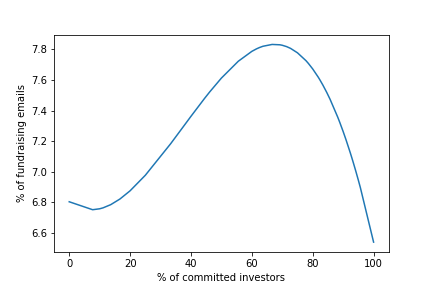
\includegraphics[width=\textwidth]{founder_rank/email_over_decided.png}
    \caption{Email Volume over \% Committed}
    \label{fig:patterns:email}
  \end{minipage}\hfill
  \begin{minipage}[t]{0.5\textwidth}
    \centering
    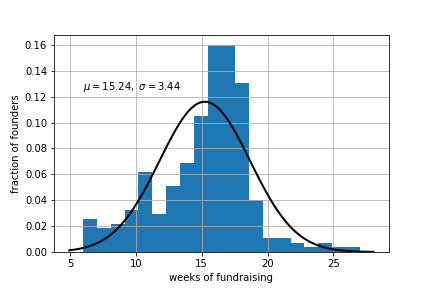
\includegraphics[width=\textwidth]{founder_rank/weeks_hist.png}
    \caption{\# Weeks Fundraising}
    \label{fig:patterns:fundraising}
  \end{minipage}
\end{figure}

\section{Baseline Ranking}

In order to evaluate any future scoring functions, we need a baseline to compare against. In the absence of a quantitative baseline scoring function, we hand-crafted a baseline ranking, incorporating our knowledge of venture capital, and the results of the research cited thus far. The goal of this baseline is to rank founders based on how likely they are to raise the largest round in the shortest period of time. We will briefly document the process of exploring features for this baseline before defining the actual scoring function.

\subsection{Potential Features}

Below are the features that were considered for the function, and our evaluation of each one for inclusion.

\subsubsection{Total funding of current round}

When available, the total amount of money raised in the current round is an excellent indicator of fundraising success, as it is normally the goal of the founder to raise as much money as possible, up to some internal maximum. This metric should definitely be included in the scoring function. Unfortunately, for many founders on the platform who are currently attempting to raise their seed rounds of funding, there might not yet be any money raised.

\subsubsection{Total funding of previous rounds}

As referenced earlier in Section \ref{chap3:tool} (p. \pageref{chap3:tool}), the First Round Capital 10 Year Project \cite{first-round-10-years} indicated much higher fundraising success rates for repeat founders. In this case, having raised money either in a previous round for the same company, or for a previous company, would give a founder the credibility and experience necessary to improve their chances for their current fundraise. We experimented including both this number, when available, as well as a binary feature indicating that this number is nonzero. Ultimately, we decided to use the raw number, as variations in this metric are significant.

\textbf{TODO: weight by average round size for the industry}

\subsubsection{Number of intro requests accepted}

While it would be useful to include a metric capturing a founder's success rate when requesting cold introductions on the VCWiz platform, there is simply not enough information for the metric we report to be indicative of anything. This follows from our earlier analysis (Section \ref{chap4:introrequests}) on why this feature saw very little usage.

\subsubsection{Number of interested investors}

A metric which is indicative of global investor interest in a company is the number of investors who have exchanged multiple emails with the founder during the timeframe of the raise. While these investors may or may not end up investing, the fact that they were interested enough to email several times is a strong signal that the founder will have options to select from when it comes time to close the round.

\subsubsection{Fraction of investors who respond}

A similar metric to the last is the percentage of investors who have emailed a founder back after the founder has initiated contact with them (either directly or through an introduction). A high value here indicates that the founder and their company are compelling enough to garner investor interest, and will have several options to select from when fundraising is over. It's also indicative of a founder's ability to reach out to investors who are a good fit for the startup.

\textbf{TODO: consider splitting cold outreach vs warm into}

\subsubsection{Average response time per investor}

The average time an investor takes to respond to a founder's email would be indicative of the investor's excitement for the founder, if all such communication happened over email and was captured by the platform. However, many founders are not using the email integrations of VCWiz, and many more will have the most crucial conversations by phone or in-person. This can create outliers which heavily skew the average and add a burdensome level of noise. Thus, this feature will not be included.

\subsubsection{Length of fundraising period}

A strong fundraise (based on our earlier criteria) is one which results in sufficient dollars being raised, in the shortest amount of time possible. Thus, the amount of time spent fundraising should be a high-signal feature: a short fundraise alone is not indicative of success, but assuming success, shorter fundraise times are better. However, our method of calculating the fundraising period is error-prone: if a founder stops using the platform, or is unsuccessful in closing their round, we will not account for this. For this reason, we omit this feature.

\textbf{TODO: use this feature?}

\subsubsection{Average sentiment of investors}

Intuitively, a high positive sentiment from an investor in an email indicates an affinity, and a strong relationship. Looking at the data on VCWiz, strong sentiment is often associated with a pre-existing relationship, often from a previous company. However, it is a very noisy source of data. Figures \ref{fig:sentiment:raised} shows the average sentiment of an incoming email during fundraising over the total money eventually raised, across all founders on the platform. Figure \ref{fig:sentiment:interested} shows the average sentiment over the number of featured investors who expressed interest in a startup during its fundraise. In both cases, we see that sentiment is a meaningless metric. We do not use this metric in our ranking function.

\begin{figure}[ht]
  \centering
  \begin{minipage}[t]{0.48\textwidth}
    \centering
    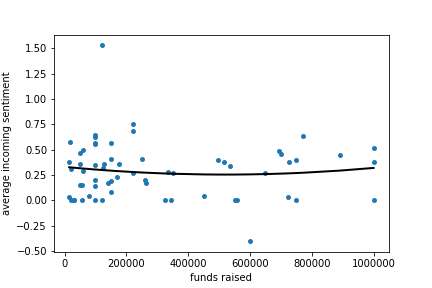
\includegraphics[width=\textwidth]{founder_rank/sentiment_over_funding.png}
    \caption{Sentiment over Money Raised}
    \label{fig:sentiment:raised}
  \end{minipage}\hfill
  \begin{minipage}[t]{0.48\textwidth}
    \centering
    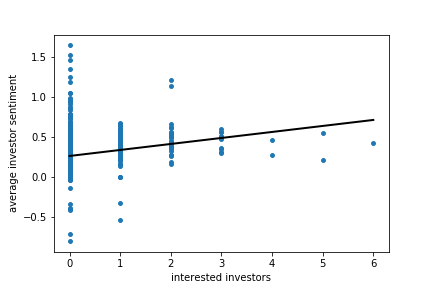
\includegraphics[width=\textwidth]{founder_rank/sentiment_over_interested.png}
    \caption{Sentiment over \# Interested}
    \label{fig:sentiment:interested}
  \end{minipage}
\end{figure}

\subsection{Evaluation}

After evaluating each of the above metrics, we drew the following conclusions. The best metric, when available, is the aggregate funding the founder has raised to date, across any company. This is the sum of the two funding-related features above. Following this, the number of interested investors is a good proxy during the fundraise, as it represents absolute interest. The email outreach success rate (fraction of investors who respond) tends to be too noisy, as it is skewed by high-profile founders who send a very small number of emails, to already-established connections. However, the number of investors who respond after being added to a wishlist on VCWiz is a very strong signal, as it indicates success with no prior relationship.

\subsection{Ranking Function}

To create a ranking function from these features, we calculate a weighted sum of sort indexes for each founder, and use the position of this score in the list of all scores as the rank. We use ranks, not absolute values, across features to account for differences in scale.

We demonstrate the scoring function in Equation \ref{eq:baseline}, where $S_{m, f}$ gives the sort index for founder $f$ when the founders are sorted by metric $m$, and $W$ is the set of (metric, weight) pairs. The final ordering of the baseline is the set of founders, sorted by this score, in ascending order (a lower score represents a higher-ranked founder).

\begin{equation}
\label{eq:baseline}
  score(f) := \sum_{(m, w) \in F} S_{m, f} * w
\end{equation}

\noindent The weights we use are found in Figure \ref{fig:nfr:baseline:weights}.

\begin{figure}[ht]
\begin{tabular}{c | c}
\textbf{Feature}           & \textbf{Weight} \\\hline
Aggregate Funding          & 4 \\\hline
\# Interested Investors    & 3 \\\hline
\# Responded From Waitlist & 2
\end{tabular}
\centering
\caption{Baseline Weights}
\label{fig:nfr:baseline:weights}
\end{figure}

This baseline, while not defensible as a ground-truth ranking for rigorous statistics, is built on sane assumptions about fundraising and venture capital. Random sampling indicates that the results are aligned with expert expectations. We will use this baseline to compare and evaluate our numerical methods for ranking, but acknowledge that it is not a perfect ranking according to the criteria we defined.

\section{Evaluation Criteria}

The next step is to define how to evaluate other ranking functions against our baseline. There are many options for evaluating ranking functions. We will discuss the options before justifying our selection. For mathematical definitions of each evaluation metric independent of our use case, we refer the reader to Section 3.2 of \cite{DBLP:journals/corr/abs-0704-3359}. These ranking functions are often used to score a permutation $\pi$ of documents given a document-set, query tuple $(D, q)$. In this case, we assume $q$ is the fixed query of founders which are most likely to succeed at fundraising, and $D$ is our list of founders.

In selecting the evaluation criteria, we imagine two relevant use-cases for our ranking functions. The first is to display a sorted list of founders to an interested party, such as an investor. The second is to use this ranking as a feature in a later process, such as enhanced matching between founders and investors (which we will explore in the next chapter).

Winner Takes All (WTA) and Mean Reciprocal Rank (MRR) are often used when displaying results based on a ranking, but both assume there is only \textit{one} top-ranked document. This does not align with either of our uses cases, so we discard them.

Discounted Cumulative Gain (DCG) takes the sum of \textit{relevances} of each founder in the ranked list (where the relevance in our case is $N - r$, with $N$ being the total number of founders, and $r$ being the rank of that founder in the baseline), weighting each founder by how early it appears in the list. We therefore get a score which increases as we put the highest-ranked founders near the start of the list, but penalizes incorrect ordering of later founders less and less. In other words, this is a metric of relative regret. This aligns well with our first use case, and provides some useful, though imperfect, information for our second.

Normalized Discounted Cumulative Gain (NDCG) simply normalizes the DCG against the number of founders in the list, so the metric can be compared across lists of different size.

Precision@n is another metric which gives preference to the top results, in this case explicitly only considering the top $n$. This metric is simply the fraction of founders in the top $n$ results that are also in the top $n$ founders of the baseline. It is a quick, useful way of evaluating a ranking for our first use case.

Root-Mean-Square Error (RMSE) is a very common error function for recommender systems (\cite{Cremonesi:2010:PRA:1864708.1864721})) which measures the differences (errors) in ranking for every founder in the list. It works very well for our second use case.

Mean Absolute Error (MAE) is another common error function, which measures the average absolute distance between a ranking and the ranking of the baseline.

Kendall's rank correlation coefficient ($\tau$) measures the ordinal association between the two lists of founders, and is often used to report on the correlation between to rankings. It roughly measures the agreement in rank over all pairs of items.

Spearman's rank correlation coefficient ($\rho$) is another measure of rank correlation. It measures the direction of association in rank between the two lists of founders.

We decided to use NDCG, Precision@n (for various values of $n$) for evaluating the quality of the rankings for the purposes of recommendation, $\tau$ and $\rho$ for calculating the rank correlation with the baseline, and RMSE and MAE for scoring the ranking as a feature to later processes. Figure \ref{fig:evaluation:formulas} shows the formulas we use for each, where $N$ is the number of founders in the list, $B$ is the baseline, $X$ is the ranking being evaluated, $R_i$ is the founder in the $i$-th position of ranking $R$, $\text{rg}(f)$ gives the rank of founder $f$ in the baseline, and $\text{sc}(R, f)$ gives the \textit{score} of founder $f$ under ranking $R$. Each ranking that we will be evaluating has a scoring function, which is in the range $[0, 1]$ for each founder. For the baseline, we assign scores by simply scaling the rank to be in this range.

\begin{figure}[ht]
\begin{equation}
  \begin{array}{c >{$\displaystyle}Sc<{$}}
    \text{\textbf{Metric}} & \text{\textbf{Formula}} \\
    \text{DCG}(X) & \sum_{i=1}^{N} \frac{2^{N - \text{rg}(X_i)} - 1}{\log_2{i + 1}} \\
    \text{NDCG}(X) & \frac{\text{DCG}(X)}{\text{DCG}(B)} \\
    \text{Precision}(X, n) & \frac{|X_{0:n} \bigcap B_{0:n}|}{n} \\
    \tau(X) & \frac{\sum_{i=1,j=1,j \neq i}^N \text{conc}(i, j, X)}{N (N - 1)} \\
    \rho(X) & 1 - \frac{6 \cdot \sum_{i=1}^N \text{drg}^2(X, B, i, i)}{N (N^2 - 1)} \\
    \text{RMSE}(X) & \sqrt{\frac{\sum_{i=1}^N \big(\text{dsc}(X, B, X_i)\big)^2}{N}} \\
    \text{MAE}(X) & \frac{\sum_{i=1}^N \big|\text{dsc}(X, B, X_i)\big|}{N}
  \end{array}
\end{equation}

\begin{align*}
 \text{drg}(X, Y, i, j) &:= \text{rg}(X_i) - \text{rg}(Y_j) \\
 \text{dsc}(X, Y, f) &:= \text{sc}(X, f) - \text{sc}(Y, f) \\
 \text{conc}(X, i, j) &:= \text{sign}\big(\text{drg}(X, X, i, j)\big) \cdot \text{sign}\big(\text{drg}(B, B, i, j)\big)
\end{align*}

\centering
\caption{Evaluation Criteria}
\label{fig:evaluation:formulas}
\end{figure}

Finally, we must define our null hypothesis, so that we can provide p-values for our rank correlations. In this case, the null hypothesis is that the correlation between the baseline and the ranking in question is 0. Thus, p gives the probability that the two uncorrelated rankings would give them same rank correlation metric value.

\section{FounderRank}

We will be ranking founders based on the information we collected on the VCWiz platform. We wish to score nodes based on graph metrics in an email graph of fundraising relationships. To do this, we first need to define a single scoring function which captures our goals. Thus we introduce FounderRank.

FounderRank is a metric in the range $[0, 1]$ that quickly communicates the strength of a founder in the global fundraising graph of founders, investors, and their mutual connections (i.e. the VCWiz Email Graph). A strong node is able to rapidly spread the word about their startup, start conversations with relevant and desirable investors, and convince investors to invest in them. These abilities are crucial for fundraising, which is in turn crucial for the survival of a startup.

Note that we are currently evaluating how well a founder can fundraise conditioned on them knowing who they would like to fundraise from. We are not tackling the issue of discovering investors, which we have touched on in the previous chapter, and will explore further in the next.

\subsection{Core Characteristics}

A combination of existing studies and our own interviews with numerous seed-stage firms reveals three intuitive properties of a founder's node in a professional or social graph which are desirable when fundraising: \textbf{importance}, \textbf{influence}, and \textbf{access}. Note that these characteristics do not take into account factors such as domain expertise, personality, and pedigree, all of which will also contribute to a successful fundraise. We are focusing exclusively on network properties for this experiment.

The first characteristic is \textbf{importance}. Importance looks at how crucial a founder is in his or her own ecosystem. This property is important as it is indicative of the founder's degree of expertise. It has been shown that in efficient professional information networks, entrepreneurs are bounced from expert to expert until they have sufficient information to answer their query~\cite{BIRLEY1985107}. The more crucial a founder is to a domain, the more access to high-quality information he or she will have. Thus, founders who have more importance are likely to be seen as a less risky investment, increasing the chances an investor responds positively to a fundraising proposal.

The second characteristic is \textbf{influence}. Influence captures how effectively a founder can effect change in their ecosystem and solicit aid from their peers. In other words, how likely are other founders to help this founder? A study on interorganizational networks of young companies found supporting evidence to the fact that ``third parties rely on the prominence of the affiliates of those companies to make judgments about their quality''~\cite{10.2307/2666998}. Founders who have high influence can leverage this to convince investors to give them funds.

The third characteristic is \textbf{access}. This is the notion of how well a founder can get in front of the investors of their choice. The more directly connected a founder is to an arbitrary investor, the more likely that investor is to respond to an inbound request (either via an introduction or cold) for funding. Additionally, a high degree of access means a founder has many options to chose from when it comes to starting conversations with investors. This follows from the more general finding that proximity in a graph to providers of valuable resources gives a node access to many viable alternatives\cite{10.2307/3069443}. This can be valuable when a founder's top choice of investor does not work out, which is often the case.

\subsection{Graph Metrics}

To quantitatively evaluate the impact of each of these characteristics, and measure their predictive capability, we need to find graph metrics which correspond to each.

For \textbf{importance}, we selected PageRank~\cite{page1999pagerank}, the canonical starting point for ranking nodes in graphs. PageRank recursively evaluates node importance by analyzing the importance of nodes which link to the node in question. It is a widely-accepted measure of node importance. We use a normalized PageRank~\cite{berberich2007comparing}, which accounts for the number of nodes and structure of the graph.

For \textbf{influence}, we selected Betweenness Centrality~\cite{10.2307/3033543}. Betweenness Centrality is the count of the number of shortest paths (over all pairs of nodes) that pass through the node in question. The rationale is that if a node is on the intro path for a pair of people, that node has influence over that pair, as it can control whether or not the introduction is made. This makes the assumption that every communication request goes along the shortest path, which is not perfectly accurate, but is sufficient for our purposes.

For \textbf{access}, we selected Closeness Centrality~\cite{FREEMAN1978215}. The Closeness Centrality of a node is inversely proportional to the node's distance from every other node. Thus, this metric measures how ``close'' a node is to the other nodes in the graph, based on shortest-path lengths, normalized for the number of nodes in the graph. The rationale is that if a node can access every other node in the graph, on average, via a short path, the node must have better access than a node that must use longer paths. Once again, this assumes that the length of the shortest path between nodes is the determiner of connection strength. Based on the data presented and cited thus fair, this is a fair assumption.

To use these metrics, we take the pre-processed graph above, and calculate the raw metric value for each node. We then normalize it as specified above, and finally scale it to be in the range $[0, 1]$. We now have a number which represents the metric for a node, relative to the other nodes in the graph, and on a standard scale. Note that we do not yet specify how to combine these metrics, we are simply calculating them.

\subsection{Naive FounderRank}

We now begin to explore ways to combine these three selected graph metric to produce a scoring function that we can compare against our baseline. The Naive FounderRank (NFR) method simply averages these three numbers, per node, to arrive at a score in $[0, 1]$.

\subsubsection{Random Model}

In order to have a model to compare against, we first start with a random model, which simply generates a score randomly and uniformly in $[0, 1]$ for each founder, then ranks them based on this score. The metrics for our random model are found in Figure \ref{fig:rand:results}.

While the random model would never be used for a serious application, it is worth noting that this way of sorting founders is not too far from the techniques used by many analysts in the real world today. The status quo at many firms involves haphazardly picking new companies to investigate based on ``gut feelings'': heuristics based on pattern-matching previous successes without any grounding in data. In one extreme case, an individual we interviewed claimed he triages companies by first sorting them alphabetically.

\begin{figure}[ht]
\begin{tabular}{c | c | c | c | c | c | c | c}
NDCG & P@5 & P@10 & P@20 & $\tau$ & $\rho$ & RMSE & MAE  \\
0.270 & 0.2 & 0.1 & 0.05 & 0.00689 & 0.0100 & 0.255 & 0.234 \\
\end{tabular}
\centering
\caption{Random Results}
\label{fig:rand:results}
\end{figure}

$\rho$ and $\tau$ have p-values of $0.808$ and $0.813$ respectively. As expected, there is essentially no correlation between the random model and the baseline.

\subsubsection{Evaluating NFR}
\label{ch5:nfr:eval}

We now move on to evaluating NFR. The first observation we made when trying to rank the founders based on NFR is that our rankings totally missed founders on the platform who are not currently fundraising, but who are known to be repeat founders who have successfully fundraised in the past. This was a result of our email graph only spanning the last year. Relationships in the venture capital world take years to build up, and we were not evaluating them over a large enough timeframe. Thus, we re-built our graph to incorporate the last five years of data, which gave us a much more comprehensive view of the ecosystem.

The below observations and conclusions are all drawn from this new graph, with up to five years of email data from 558 founders.

We sorted the founders in our original list by their NFR score, and then evaluated this ranking based on our earlier-established criteria. The results are shown in Figure \ref{fig:nfr:results}.

\begin{figure}[ht]
\begin{tabular}{c | c | c | c | c | c | c | c}
NDCG & P@5 & P@10 & P@20 & $\tau$ & $\rho$ & RMSE & MAE  \\
0.448 & 0.2 & 0.3 & 0.2 & 0.484 & 0.673 & 0.0827 & 0.0637 \\
\end{tabular}
\centering
\caption{NFR Results}
\label{fig:nfr:results}
\end{figure}

The p-values for $\tau$ and $\rho$ are respectively $10^{-65}$ and $10^{-75}$.

\subsubsection{Discussion}

As expected, the naive model easily and confidently beats the random model on every metric. While this is intuitive (there must be \textit{some} information in this graph), it is important to point out that even such a simple, naive model can best a standard seen often in venture today. If the goal is to use this ranking to surface interesting founders, NFR is an acceptable solution, albeit not great. The precision is still too low to be considered truly valuable. As a feature, the rank correlation observed in NFR is impressive. The degree to which naively combining graph metrics gives a score correlated to the baseline indicates how important the founder's position in their social-professional graph is.

We can interpret $\tau$ as saying that there is reasonable agreement between the rankings presented by NFR and the baseline, and $\rho$ as saying the direction of association in the rankings is positive, and significantly so: more often than not, the ranking of NFR tends to increase when the baseline does the same.

A final observation is that, as expected, all of the relative regret metrics increased after rebuilding the graph over a longer time period. It is easier to identify strong founders when relationships over a long period of time can be taken into account. Founders in the middle of the ranking largely stayed in the same position, as no new information was revealed about them.

\subsubsection{Edge Weights}

One interesting experiment we considered was using the frequency of emails exchanged between two nodes as an edge weight. Running the same metric algorithms on this new weighted graph should render even more accurate data about relationships, the position of a given node, and therefore the strength of the founder in the graph. Unfortunately, there is a significant amount of work involved in re-writing the metric algorithms to incorporate edge weights, and we did not have the time to explore this. We leave it as future high-potential work.

\subsection{Weighted FounderRank}

The next model we experimented with is a linear combination of the three graph metrics, as determined by a simple linear regression, using the hand-crafted baseline ranking as labels. We fit a standard linear regression model to the baseline ranking, using each of the three graph metrics as a feature. We get an $R^2$ value of $0.39$, with evaluation metrics as shown in Figure \ref{fig:wfr:results}. The change in metrics is negligible, with NDCG, $\tau$, and $\rho$ increasing slightly, but our error functions (RMSE and MAE) also increasing slightly.

\begin{figure}[ht]
\begin{tabular}{c | c | c | c | c | c | c | c}
NDCG & P@5 & P@10 & P@20 & $\tau$ & $\rho$ & RMSE & MAE  \\
0.449 & 0.2 & 0.3 & 0.2 & 0.490 & 0.680 & 0.103 & 0.0787 \\
\end{tabular}
\centering
\caption{WFR Results}
\label{fig:wfr:results}
\end{figure}

More interestingly, we can examine the effect on our evaluation metrics and $R^2$ by using different combinations of the three graph metrics, with the goal of determining their relative importance.

\subsubsection{Sole Metrics}

If we rank our founders based solely on their PageRank, we get abysmal evaluation metrics, with the exception of NDCG, which is significantly higher at $0.527$. This implies that if our sole concern was surfacing the best few founders from the batch, sorting by PageRank would be a good option. This corroborates our conclusions from extending the timeframe over which the graph is built: the best founders often are well-embedded and have built up strong relationships over years, giving them a high PageRank.

If we rank solely based on a founder's betweenness, every metric is strictly worse. The $R^2$ value of the regression actually goes negative, indicating that this metric alone is a very poor model of a founder's potential for fundraising success. Furthermore, a founder's betweenness is highly correlated with their PageRank (a Pearson correlation coefficient of $0.913$), making it unnecessary to ever consider it.

Finally, if we rank solely on closeness, we end up with a lower NDCG (at $0.375$), but increased P@5 ($0.4$) and $\tau$ ($0.498$). The RMSE increases to $0.135$. The conclusion here is that how much access a founder has in the graph can offer a marginally better ranking in isolation, though at the cost of less accurate individual scores. For ranking, it appears that closeness explains more of the optimal ranking than any other metric, and this is supported by the relatively close $R^2$ value of $0.348$. While it is far from a perfect model, a node's closeness centrality in the email graph explains about 35\% of the variance of a hand-tuned ranking of the founders in the graph.

Our conclusion from testing these individual metrics is that access is most important aspect of a founder's node in the graph, but a sufficiently high importance (PageRank) can compensate for a lower closeness centrality.

\subsubsection{Optimal Combination}

Based on the above, the optimal combination of features is some linear combination of PageRank and Closeness Centrality. We ran another linear regression with these two features, resulting in a model that has similar evaluation metrics, save for the highest NDCG seen yet ($0.533$). Adding PageRank to Closeness Centrality in our model brings $R^2$ to $0.391$, a $12.8$\% increase.

\subsubsection{Conclusion}

The goal of these experiments on the VCWiz Email Graph was to explore whether the data stored in the graph structure and relationships could improve the process of predicting a founder's ability to fundraise, for use in the founder-investor matching process by both humans and other models. We have shown that there is signal in our selected graph metrics of founder nodes.

Through these experiments, we have determined that graph metrics alone can do a good job scoring founders. The rankings are not perfect, and can only explain about 40\% of the variance seen in the baseline they are compared against, but they significantly best the status-quo of an effectively random model, and have considerable rank correlation with the baseline ($\rho = 0.680$, p $\approx 0$). Upon examining the individual graph metrics, we see that Closeness Centrality, which corresponds to a founders ``access'' in the graph, is the driving factor, with exceptions in the case of very successful founders who have extraordinary PageRank. We also find that Betweenness Centrality, which indicates a founder's influence over introductions, is a near-meaningless metric, with information that is captures almost entirely by PageRank.

The takeaway of access being a driving factor to founder fundraising success further motivates our work on the VCWiz platform. We've demonstrated that founders who have a short average distance to investors tend to see success fundraising. A stated goal of the platform is to increase founders' access to investors, a demonstrably high-impact outcome. We accomplish this by helping founders discover and understand investors who are within reach of their network, and facilitate connections which add edges in the relationship graph. VCWiz enables these connections for all founders, enshrining equality in what is otherwise an insider's game.

\section{FounderRank with Investment Data}

The next experiment explores whether the conclusions of the FounderRank experiment hold true on the global graph of venture investments. If so, we wish to explore whether adding global investment data to the VCWIz Email Graph can augment it and provide even better rankings.

We begin with considering the public graph of venture fundings, as reported by VCWiz. At the time of writing, this database contains $288,720$ founders, $92,843$ investors, and $57,131$ investments. For an overview of how this data is collected, see Section \ref{ch4:data} (\pageref{ch4:data}). The graph is constructed by creating a node for every founder and investor on the platform, each tagged as such. For each instance of an individual investor investing in a founder's company (see Section \ref{ch4:partners} for an overview of how this information is inferred), two edges are added: one from the founder to the investor, and one from the investor to the founder.

\subsection{Baseline}

As before, there is no ground-truth ranking of the founders in this graph, so we need to generate a baseline. We will focus on public metrics involving the past experience of the founders, as well as the aggregate money they have raised. We rely on the work done in \cite{2017arXiv170604229H} as justification for selecting these metrics.

\begin{quote}
We see that the top non-sector features are related to the past experience of the leadership (executive acquisition, executive IPO, advisory IPO, leadership age). The investor feature maximum acquisition fraction is also one of the top non-sector features. This suggests that companies with experienced and successful leadership and investors have increased drift which results in a higher exit probability.
\end{quote}

The features we selected are Job IPO, Job Acquired, Executive IPO, Executive Acquired, Advisory IPO, and Advisory Acquired. These features track initial public offerings and acquisitions across any company the founder has worked at, started, or advised. The specific feature we use is the sum of all these numbers. We call this feature Affiliated Exits.

Using the same process as before (a combination of manual inspection, sane priors about venture capital, and consulting experts), we arrived at the baseline weights shown in Figure \ref{fig:fri:baseline:weights}. We use the same scoring function construction as in Section \ref{ch5:nfr:eval}. We will also use the same evaluation metrics.

\begin{figure}[ht]
\begin{tabular}{c | c}
\textbf{Feature}   & \textbf{Weight} \\\hline
Affiliated Exits   & 4 \\\hline
Aggregate Funding  & 1
\end{tabular}
\centering
\caption{Baseline Weights}
\label{fig:fri:baseline:weights}
\end{figure}

The rationale for these weights follows from the metrics from \cite{2017arXiv170604229H} which have been shown to correlate with a founder's success rate, including ability to successfully fundraise. We additionally add the Aggregate Funding feature from the last experiment, to acknowledge that founders who have raised a large amount of capital in the past are more likely to be trusted as stewards of capital in the future.

One interesting observation about this baseline is that rewarding a large number of exists gives us a ranking that surfaces many founders who are now investors. This aligns well with career paths seen in the venture world: founders who take a company from birth to exit have experience that is highly sought-after in investors.

\subsection{Random Model}

Much as before, a random model shows the expected characteristics with all our evaluation criteria. There is no rank correlation with the baseline.

\subsection{Optimal FR+I Model}

The best linear combination of graph metrics for the global funding graph tells a very different story than that of the VCWiz Email Graph. In this case betweenness, which we previously identified as a near-useless metric, has a large negative coefficient when included, with a model that is effectively the same as omitting it altogether. The remaining combination of PageRank and closeness still gives us an abysmal result: an $R^2$ of $-0.268$, with a $\rho$ of $0.192$ (with a p-value of effectively $0$). We see that there is no way to give a reasonably good ranking function based on these three graph metrics on the graph of venture fundings, implying that this graph carries very different information from the social-professional email graph.

\subsection{Broader Venture Ecosystem}

We further experimented with the graph of funding data, augmenting it with data about both co-founding relationships (founder-founder) and co-investing relationships (investor-investor). The co-investing relationships (an edge between a pair of investors if and only if those two investors have participated in the same funding round of a company) did not significantly improve our models, but the co-founding relationships did.

In this new graph of investment and co-founding relationships, the best model is the one that solely uses the closeness metric. This is consistent with all our previous conclusions. With this model, we get a $\rho$ of $0.357$. While this is not as strong a correlation as the email graph was, it still shows a similar result. This result is consistent, as we expect there to be less information in a graph of public investment and cofounding data than there is in a social-professional graph that reveals the many conversations which do not end in an investment or new company.

\subsection{FR+I with Email Data}

We have shown so far that the data in the global funding graph alone is not sufficient to show any meaningful correlation. However, we know that the private email graphs of founders \textit{do} have predictive power. To explore whether or not there is any value in the global funding graph's relationships in the context of ranking founders, we took the VCWiz Email Graph and overlaid the graph of investment and co-founding relationships from the previous section.

The results confirm what we expected: the email graph contains sufficient information to predict a founder's fundraising ability, and given this, the public funding graph adds information which makes increases the correlation of the model's ranking with the baseline. Upon adding the public graph nodes and relationships, we see an increase in $\rho$ from $0.680$ to $0.695$, and a doubled P@5 of $0.4$.

\subsection{Conclusion}

Our conclusion from the above experiments is that the public graph of venture funding relationships does not provide adequate information on social-professional networks to draw conclusions about the strength of a founder (and his or her ability to fundraise). While private graphs, such as the VCWiz Email Graph, which capture \textit{all} communication between founders, investors, and their intermediaries can be useful in evaluating and characterizing founders, public data falls short. We believe this is in part due to private conversations including those which do not culminate in a fundraising relationship; while an investor may not invest in a founder, a strong relationship might still exist which can be leveraged at a later date. Furthermore, public data makes it difficult to infer social friendships which are captured in emails, and might be crucial to introductions. This public data can, however, still be used to successfully augment an existing private graph with additional relationships from venture investments past and present. Since the public graph adds relevant relationships to those implied by emails, we see an increase in the efficacy of the email-based graph when augmenting it with the global funding graph.

\section{InvestorRank}

For this final experiment, we explore the value in calculating the same graph metrics considered above for the investors themselves.

\textbf{TODO: run the numbers and see if it makes sense to include, using co-investment edges}

\textbf{TODO: baseline ranking of sum of investments which have exited}
% (don't want to use exit amounts bc outliers skew everything)

% See if it makes sense to run these graph metrics for investors on the graph themselves. See is there if correlation between InvestorRank and FounderRank of the founders invested in by that investor. How to do correlation calculation for many to many -- Pairwise?

% Future: Given that the FounderRank metric seems indicative of a founder's ability to raise, and that raising is a crucial part of keeping a company alive, does ranking investors by the mean founder rank of the founders they've invested in give us a reasonable ranking of investors? Manually inspect it, also compare it to baseline, which can use features like \# of exists, total follow-on raised, and total valuation at IPO sum.

